% =============================================================================
% Part I, Chapter 1: The Origin
% =============================================================================
\chapter{The Origin}\label{ch:origin}

\section{The Founding Motivation: Compression Meets Intervention}

Every empirical research program begins inside a specific technological moment. By late 2026, open-weight instruction-tuned large language models (LLMs) in the 3-billion to 14-billion parameter regime were routinely deployed on commodity laptops, edge servers, and local clinical or industrial workstations using post-training weight quantization (PTQ). Formats from the \texttt{GGUF} ecosystem---most notably 4-bit K-quantization (\texttt{Q4\_K\_M}) and aggressive 2-bit or 3-bit variants (\texttt{Q2\_K}, \texttt{Q3\_K\_M})---reduced memory footprints by $65\%$ to $82\%$ relative to IEEE half-precision (\texttt{F16}), allowing practitioners to run models locally via \texttt{llama.cpp} without datacenter accelerators.

Standard compression benchmarks generally reassured practitioners that 4-bit quantization preserved perplexity and multiple-choice accuracy within one to two percentage points of \texttt{F16}. Yet emerging studies in 2025 and 2026 had begun warning that surface benchmark stability could conceal sharper failures on multi-step mathematical reasoning, long-context state tracking, and parametric recall \citep{liu2025hurts,li2025meets,zhang2025compression,lian2026inflates,alimaskina2026extreme}. Concurrently, a separate literature on causal reasoning in LLMs was asking whether language models could genuinely operate on Judea Pearl's second rung of the Ladder of Causation---predicting the effects of \emph{interventions} $\Prob(Y \mid \doop(X=x))$ when confounding variables distort raw observational correlations $\Prob(Y \mid X=x)$---or whether models merely matched semantic templates and memorized domain heuristics \citep{jin2023cladder,kiciman2023causal,yu2025causaleval,wang2026causalflip}.

Project \textbf{CausalFade} was conceived at the intersection of those two questions. Its earliest recoverable record in Git history is commit \nolinkurl{4e2fe4f53370c05878476ed0363bf472fcd34d17}, authored on October 28, 2026 (\texttt{2026-10-28T07:18:34+05:00}), which committed the initial fourteen-paper literature archive (\texttt{literature review/}) and executive research scoping document (\texttt{literature review/EXECUTIVE\_SUMMARY.md}). As documented in \texttt{EXECUTIVE\_SUMMARY.md} and the earliest root \texttt{README.md}, CausalFade originated as a rigorous university research project investigating a specific, high-stakes failure mode:

\begin{quote}
\emph{When an AI agent is compressed to fit local hardware via post-training quantization, does its capacity to separate genuine causal effects from spurious confounding associations ``fade'' faster than its general fluency---causing quantized agents to recommend harmful interventions whenever historical correlation points in the wrong direction?}
\end{quote}

Figure~\ref{fig:timeline} situates this founding moment at the start of the twenty-nine-day arc that followed.

\begin{figure}[htbp]
  \centering
  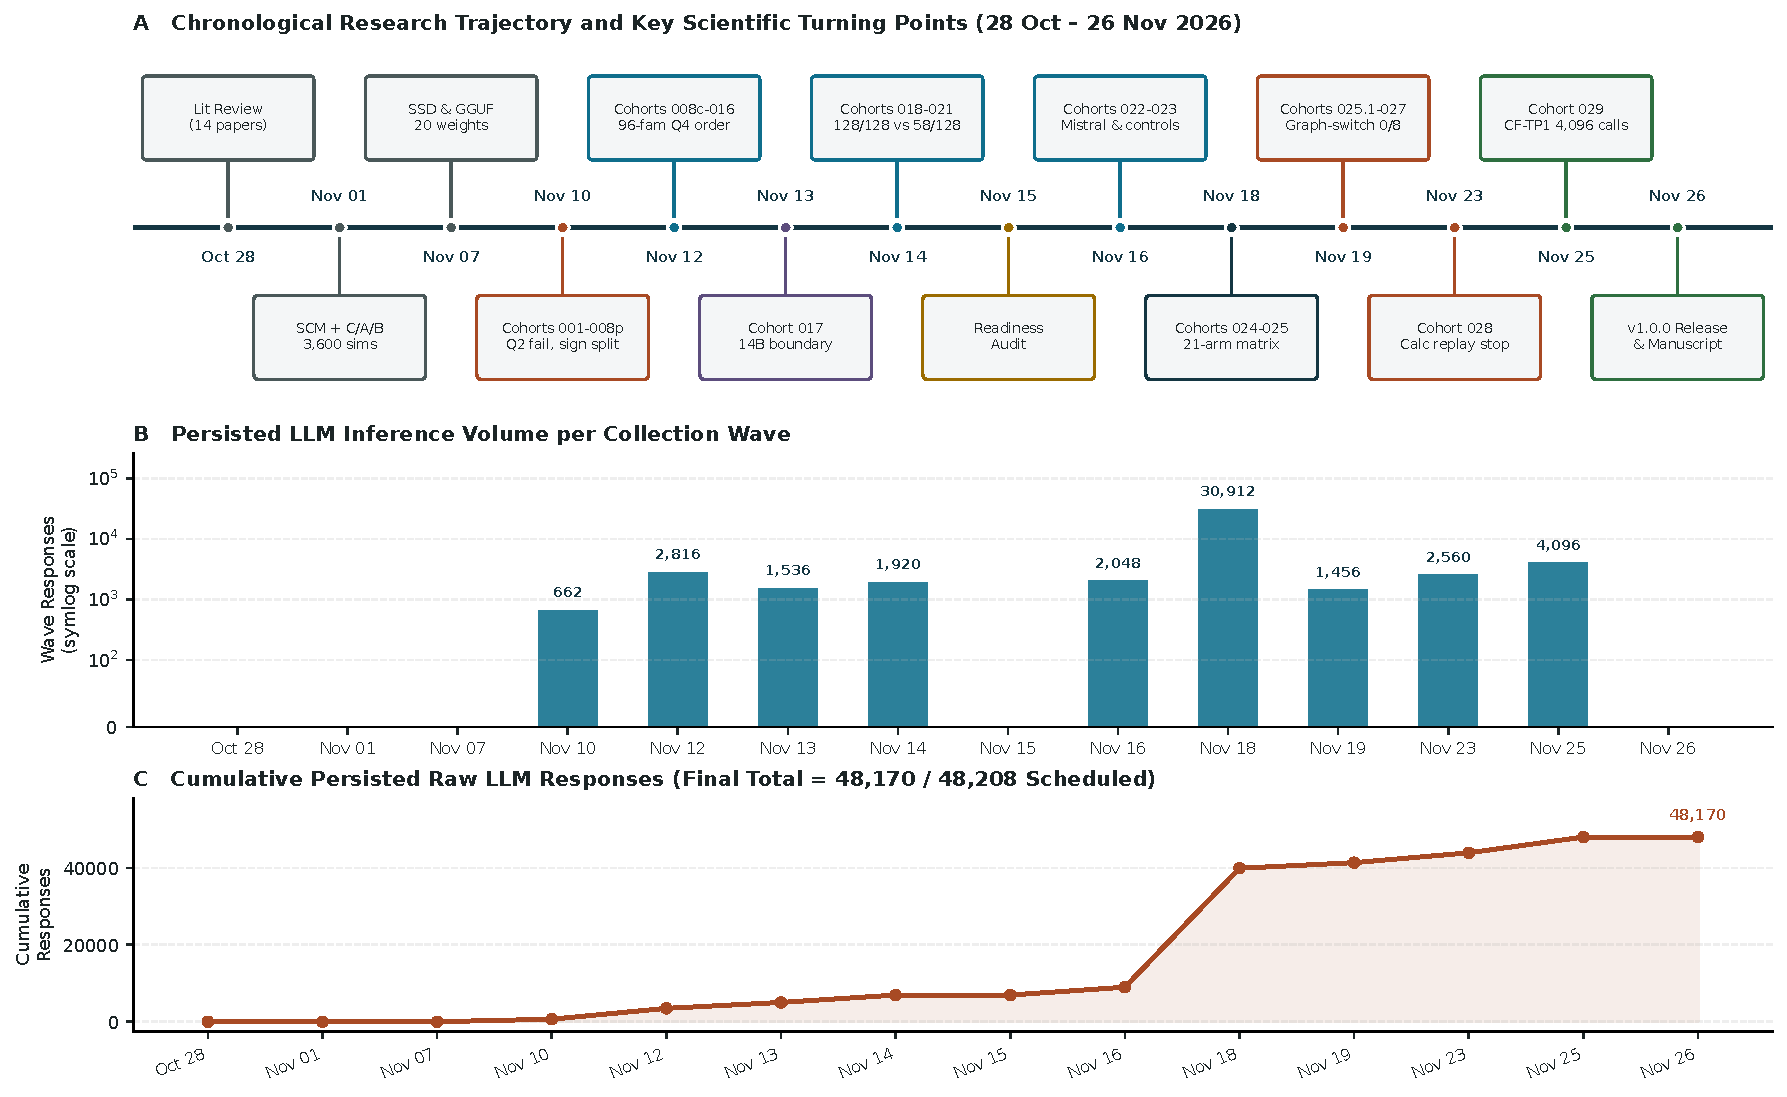
\includegraphics[width=\textwidth]{figures/fig01_research_timeline.pdf}
  \caption{Chronological overview of Project CausalFade across its 11 research phases (October 28 -- November 25, 2026; 320 commits, 30 cohorts plus pre-LLM synthetic validation, and $48{,}208$ scheduled inference requests).}
  \label{fig:timeline}
\end{figure}

\section{Why Causal Reasoning and Quantization Were Paired}

From a scientific standpoint, pairing causal identification with weight quantization was not an arbitrary combination of trendy topics; it rested on a plausible cognitive and computational asymmetry:

\begin{enumerate}
  \item \textbf{Associative shortcuts are cheap; causal adjustment is compositional.} In a confounded observational table where an upstream variable $Z$ (such as initial machine severity or patient baseline risk) drives both operator action $X$ and outcome $Y$, raw marginal association $\Prob(Y=1\mid X=1) - \Prob(Y=1\mid X=0)$ requires comparing two coarse summary tendencies. By contrast, Pearl's backdoor adjustment formula,
  \begin{equation}
    \Prob(Y=1 \mid \doop(X=x)) = \sum_{z \in \{0,1\}} \Prob(Y=1 \mid X=x, Z=z)\,\Prob(Z=z),
    \label{eq:origin_backdoor}
  \end{equation}
  requires (i) recognizing the causal graph structure $Z \to X, Z \to Y, X \to Y$, (ii) resisting the misleading marginal contrast, (iii) stratifying by $Z$, and (iv) weighting stratum-specific rates by target marginal shares $\Prob(Z=z)$ rather than treatment-conditioned shares $\Prob(Z=z\mid X=x)$.
  \item \textbf{Quantization introduces structured numerical perturbation into attention and MLP weights.} Post-training quantization maps continuous 16-bit floating-point weight blocks into coarse integer grids ($2$ to $8$ bits per weight). Recent work by \citet{marcuzzi2026bias} showed that quantization can amplify pre-existing distributional biases, while \citet{nwaiwu2025compressed} had published the only prior study explicitly combining quantization with causal benchmarks (\texttt{CLadder}), reporting accuracy drops at 4-bit precision.
  \item \textbf{The practical safety hazard of silent associative fallback.} If a heavily quantized model crashes into unreadable gibberish (as \texttt{Q2\_K} eventually did in Cohort~001), downstream software rejects the malformed output immediately. The far more dangerous failure mode hypothesized at project inception was \emph{silent schema-valid reversal}: a quantized model returning clean, syntactically valid JSON (\texttt{\{"activate": 1\}}) that confidently endorses a harmful action because quantization eroded multi-step backdoor adjustment while leaving associative pattern-matching intact.
\end{enumerate}

\section{The Initial Research Question and Prospective Hypothesis}

In its earliest formalization (\texttt{literature review/EXECUTIVE\_SUMMARY.md}, commit \texttt{4e2fe4f}, and \texttt{docs/STATISTICAL\_ANALYSIS\_PLAN.md}, commit \texttt{6ab18d2}), the project posed the following primary question:

\begin{definition}[Founding Research Question, October 28 -- November 1, 2026]
Does aggressive post-training quantization ($p \in \{\text{\texttt{Q8\_0}}, \text{\texttt{Q4\_K\_M}}, \text{\texttt{Q2\_K}}\}$) selectively increase an instruction-tuned LLM's vulnerability to confounding associations on interventional decision tasks relative to its unquantized half-precision (\texttt{F16}) reference?
\end{definition}

To operationalize this question, the researchers constructed synthetic binary structural causal worlds crossed in a $2\times 2$ design over two binary cues:
\begin{itemize}
  \item the \textbf{true interventional sign} $T \in \{0,1\}$, where $T=1$ iff $\ATE = \E[Y\mid \doop(X=1)] - \E[Y\mid \doop(X=0)] > 0$, and
  \item the \textbf{naive observational association sign} $S \in \{0,1\}$, where $S=1$ iff $\RD_{\mathrm{obs}} = \Prob(Y=1\mid X=1) - \Prob(Y=1\mid X=0) > 0$.
\end{itemize}
In \emph{aligned} items ($T = S$), causal adjustment and naive association recommend the same binary action. In \emph{conflict} items ($T \neq S$, a Simpson's reversal), naive association recommends the causally harmful action. Defining the within-precision conflict penalty as
\begin{equation}
  \mathrm{ConflictPenalty}(p) = \mathrm{Acc}_{\mathrm{aligned}}(p) - \mathrm{Acc}_{\mathrm{conflict}}(p),
\end{equation}
the founding prospective hypothesis (\texttt{H01} in our Hypothesis Ledger) predicted a positive quantization-by-conflict interaction:
\begin{equation}
  \Delta(p) = \mathrm{ConflictPenalty}(p) - \mathrm{ConflictPenalty}(\text{\texttt{F16}}) > 0.
  \label{eq:origin_delta}
\end{equation}

Notably, even at commit \texttt{4e2fe4f}, the researchers made a mature scoping decision (\texttt{D01} in \texttt{literature review/EXECUTIVE\_SUMMARY.md}): although early brainstorming had used the vivid metaphor of quantization ``severing causal circuits,'' the literature synthesis explicitly warned that behavioral prompts cannot identify internal neural circuits without activation patching or mechanistic interpretability. Accordingly, CausalFade prospectively restricted its claims to \emph{behavioral interventional competence} from day one.

\section{Original Assumptions---and How Reality Tested Them}

Looking back from the completed archive, the founding design rested on five implicit assumptions, every single one of which would soon fail empirically:

\begin{enumerate}
  \item \textbf{Assumption 1 (Reference Competence):} Unquantized \texttt{F16} instruction-tuned models ($3\text{B}$--$8\text{B}$) can reliably solve confounded interventional decision problems, providing a non-degenerate ceiling from which quantized models might ``fade.'' \emph{Reality:} Even \texttt{F16} models hovered near chance ($43\%$--$55\%$) on properly controlled causal decisions whenever surface shortcuts were removed.
  \item \textbf{Assumption 2 (Parser Neutrality):} Strict JSON schema enforcement treats \texttt{F16} and quantized models symmetrically. \emph{Reality:} In Cohort~001, \texttt{F16} wrapped valid JSON in Markdown fences $100\%$ of the time ($0/64$ strict accuracy), whereas \texttt{Q4\_K\_M} occasionally omitted fences, and in Cohort~024 \texttt{Llama-3.1-8B Q4\_K\_M} suffered $448$ length-capped verbose failures exclusively on noncausal controls.
  \item \textbf{Assumption 3 (Unbiased Action Priors):} Errors on conflict items reflect reliance on confounding association $S$ rather than unconditional preference for \texttt{activate=1} or \texttt{activate=0} or first-listed options. \emph{Reality:} Across nearly every cohort, models exhibited massive unconditional action biases (e.g., $63/64$ \texttt{activate=1} in Cohort~001 \texttt{F16}, $64/64$ \texttt{activate=0} in Cohort~002 \texttt{F16}, $995/1{,}024$ \texttt{activate=1} in Cohort~029 causal transfer, and $256/256$ first-option selection in Cohort~024 \texttt{Mistral F16}). Under a constant action policy, aligned and conflict accuracy are both exactly $50\%$, driving $\mathrm{ConflictPenalty}(p)$ artificially to $0$!
  \item \textbf{Assumption 4 (Internal Consistency Between Math and Action):} If a model computes the right negative ATE ($\widehat{\tau} < 0$), it will choose \texttt{activate=0}; if it computes $\widehat{\tau} > 0$, it will choose \texttt{activate=1}. \emph{Reality:} Cohorts~002, 006, and 007 uncovered a striking numeric-to-action dissociation in which \texttt{Qwen2.5-3B F16} computed the correct ATE sign on $61/64$ ($95.3\%$) of formula-assisted prompts while outputting \texttt{activate=0} on $64/64$ ($100\%$).
  \item \textbf{Assumption 5 (Absence of Numerical Magnitude Shortcuts):} Crossing $T$ and $S$ suffices to prevent noncausal shortcuts. \emph{Reality:} Unless numerical effect distributions are matched across studies and roles, deterministic source-blind rules (such as picking the smaller printed $|\text{on}-\text{off}|$ gap in Cohort~016) can achieve $100\%$ accuracy without reading causal provenance at all.
\end{enumerate}

\section{Original Objective vs.\ Eventual Scientific Contribution}

To read CausalFade honestly, one must hold two truths in view from the outset (Figure~\ref{fig:q_evolution}):

\begin{figure}[htbp]
  \centering
  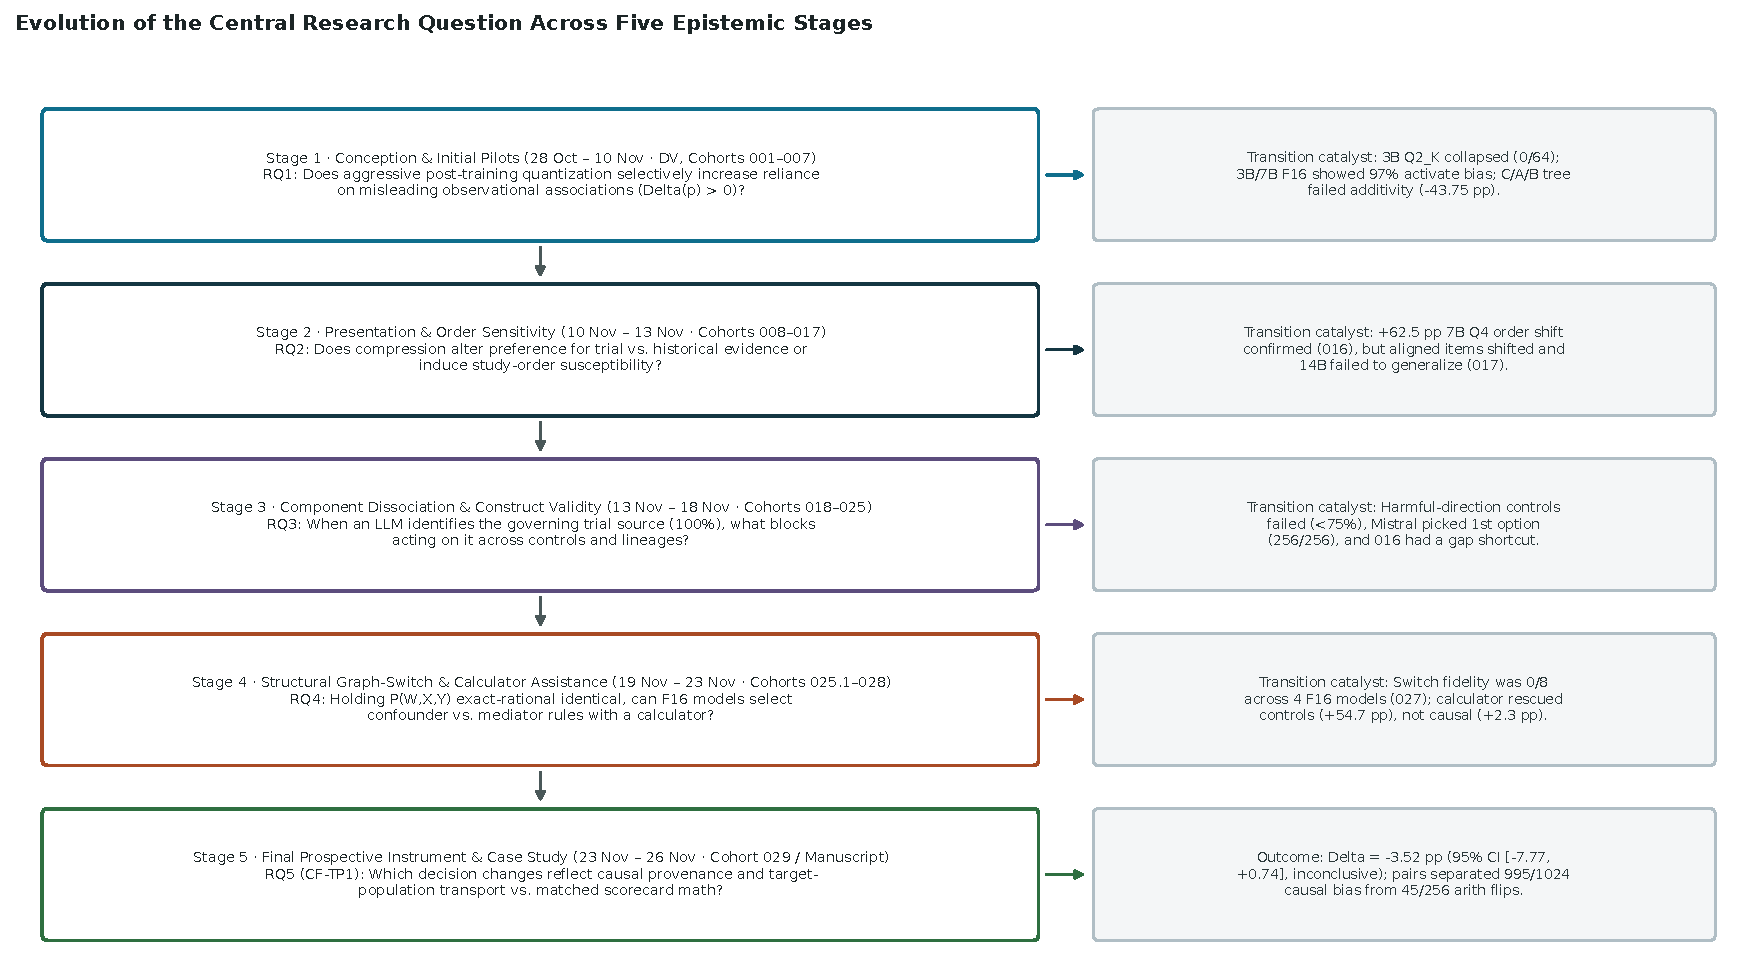
\includegraphics[width=\textwidth]{figures/fig02_question_evolution.pdf}
  \caption{Six-stage evolution of CausalFade's central research question, tracing how empirical anomalies forced the program from a quantization-degradation hypothesis (\texttt{RQ1}) to a general diagnostic framework for target-population causal transport and shortcut elimination (\texttt{RQ6}).}
  \label{fig:q_evolution}
\end{figure}

\begin{itemize}
  \item \textbf{What CausalFade originally hoped to demonstrate:} A clean dose--response curve showing that as GGUF precision drops from \texttt{F16} to \texttt{Q8\_0}, \texttt{Q4\_K\_M}, and \texttt{Q2\_K}, causal sensitivity $C$ decays while associative reliance $A$ rises.
  \item \textbf{What CausalFade actually discovered and contributed:} Selective quantization degradation of causal reasoning was \emph{not} established. Instead, through twenty-nine iterative cohorts of falsification and repair, CausalFade demonstrated why standard single-item LLM causal evaluations are pervasively confounded by action priors, option-order policies, numeric shortcuts, and baseline aggregation failures---culminating in \textbf{CF-TP1} (Cohort~029 and \texttt{manuscript/}), an exact-rational, $162$-policy-audited, paired reversal-and-retention benchmark for target-population causal transportability with matched noncausal arithmetic controls.
\end{itemize}
